\chapter{Виконання лабораторної роботи} 
\label{chapter:first}

\section{Керування горінням світлодіода за допомогою Arduino Uno}

Оскільки таке тривіальне завдання як "поморгати" світлодіодом виконується вкрай просто (вмонтована бібліотке blink), воно не потребує жодних додаткових пояснень.

\section{Створення приладу для вимірювання освітленності за допомогою Arduino Uno}

% \subsection{Структура проекту \LaTeX{}}
Перша частина лабораторної роботи стосується досить простого завдання: використовуючи певний набір компонентів, скласти прилад, який буде оцінювати ступінь освітленності у приміщенні.

У роботі було використано наступні елементи: плата Arduino Uno, кабель usb - micro-usb, світлодіодний прогрес бар (розпіновка завантажена на репозиторій), фоторезистор, ящик із резисторами всіх відтінків. Із цього всього добра було складено схему, зображену на (рис. \ref{fig:shema1}). По суті, схема являє собою подільник напруги, до виходу якого підключений аналоговий вхід A0.

\begin{figure}[h]
\center{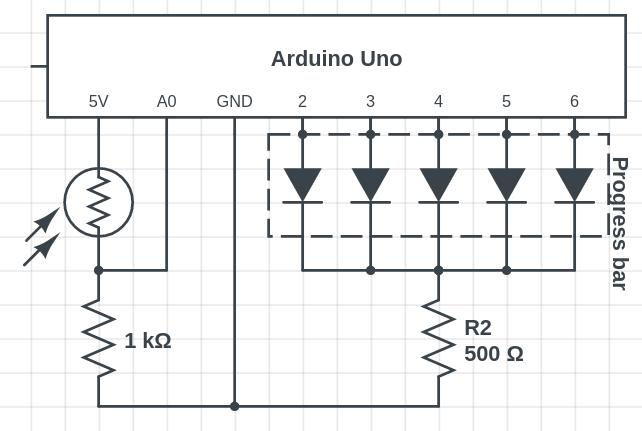
\includegraphics[width=0.6\linewidth]{shema.jpg}}
\caption{Схема підключення основних елементів схеми. Виходи 0 та 1 навмисно не використовувалися, аби зберегти можливість безпершкодного користування протоколом UART.}
\label{fig:shema1}
\end{figure}

\begin{figure}[h]
\center{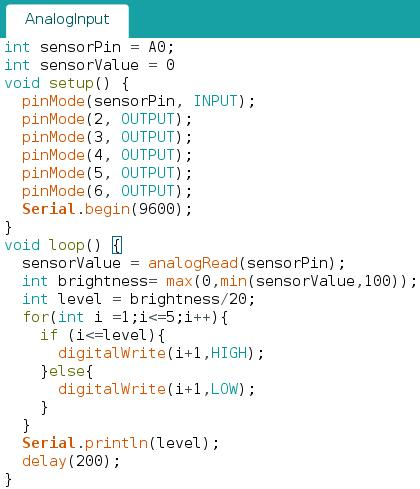
\includegraphics[width=0.5\linewidth]{code.jpg}}
\caption{Код програми мікроконтролера.}
\label{fig:code1}
\end{figure}

На практиці виявилося, що напруга на вході в ардуінку коливалася від $0$ до $\approx 100/1024 * 5 V \approx 0.5 V$, в залежності від освітленності. Очевидно, що розширити цей діапазон можна підбором резисторів інших номіналів. Але, зважаючи на лінь виконавців даної лабораторної роботи, було прийнято рішення програмно (рис. \ref{fig:code1}) врахувати цю особливість. Як показала практика, навіть такий похабний підхід дає непогані результати. (файл progressbar.mov на гітхабі)

Окрім того, автор хотів би підмітити потребу у макетних платах, із окремо виведеними лініями + та GND. Справді, використовувати 4 зайві перемички аби підтягнути всі ножки прогресбару до землі - не найприємніша справа, яка до того ж псує зовнішню простоту схеми.

\section{Керування генератором сигналів DDS 9850 за допомогою Arduino nano}

У другій частині роботи нам було запропоновано прошити arduino nano, що керувала генератором сигналів dds 9850, та дослідити сигнал, який буде створювати останній. Оскільки потрібна схема вже була зібрана на макетній платі, та зафіксована прекрасним припоєм, що остив після пайки, нам залишилося лише завантажити прошивку у контролер, що звісно супроводжувалося головним болем, викликаним налаштовуванням IDE під arduino nano. Однак, не зважаючи ні на що, робота була доведена до кінця. Тож було досліджено сигнал із виходів $sina,sinb,qp,qa$ при частотах $\nu = 100 Hz$, $\nu = 500 Hz$. Відповіді результати показані на відеороликах (gen1.mov gen2.mov)